\subsection{Configuration Editor}
\writer{Albert, Monica}

The Configuration Editor is a component that will work as a connector between the Petri net editor (Section \ref{sec:sf-petrinet}), the Geometry editor (Section \ref{sec:sf-geometry}) and the Appearance editor (Section \ref{sec:sf-appearance}). 

The editor will allow the user to load the corresponding files, created in the previous editors, that will make it possible for the simulation to be started. In order to use the Configuration Editor, the user has to \textit{create} a new or \textit{load} an existing appearance file he/she wants to edit.

\subsubsection{Functional Requirements}

\begin{enumerate}
	\item The Configuration Editor \textbf{shall} allow the user to load a Petri net doc file as a resource.
	\item The Configuration Editor \textbf{shall} allow the user to assign the loaded Petri net doc file as a value to the Configuration's Petrinet property. 
	\item The Configuration Editor \textbf{shall} allow the user to load a Geometry file as a resource.
	\item The Configuration Editor \textbf{shall} allow the user to assign the loaded Geometry file as a value to the Configuration's Geometry property.  
	\item The Configuration Editor \textbf{shall} allow the user to load an Appearance file as a resource.
	\item The Configuration Editor \textbf{shall} allow the user to assign the loaded Appearance file as a value to the Configuration's Appearance property. 
	\item The Configuration Editor \textbf{shall} allow the user to start a simulation with the referenced Petri net, Geometry and Appearance resources.
	\item The Configuration Editor \textbf{shall} allow the user to validate that all the needed files have been loaded.
	\item The Configuration Editor \textbf{shall} allow the user to save a Configuration file.
\end{enumerate}

\subsubsection{Use cases}

The features described above are shown in the following use case diagram Figure~\ref{fig:use-cases-configuration}.

\begin{figure}[htp]
\begin{center}
  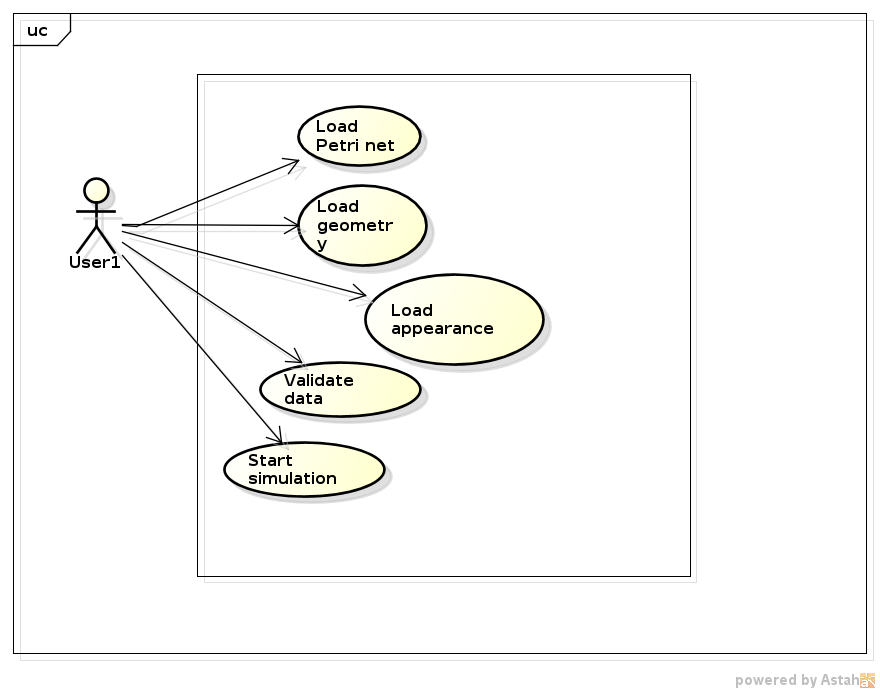
\includegraphics[width=0.5\textwidth]{image/uc-configuration.png}
  \caption{Use cases for the Configuration Editor}
  \label{fig:use-cases-configuration}
\end{center}
\end{figure}